
\section{Resultados}

\subsection{problema 1. Intervalos de Confianza por mes}




\section*{Análisis de ventas - Tienda Santa Ana}

\begin{longtable}{@{}lccc@{}}
\toprule
\textbf{Mes}       & \textbf{Ventas promedio} & \textbf{IC 95\%}               & \textbf{IC 99\%}               \\
\midrule
Enero       & \$16,311.30 & [\$15,223.36, \$17,399.25] & [\$14,846.34, \$17,776.26] \\
Febrero     & \$17,901.85 & [\$16,716.43, \$19,087.26] & [\$16,301.13, \$19,502.57] \\
Marzo       & \$20,169.85 & [\$19,189.30, \$21,150.41] & [\$18,849.50, \$21,490.21] \\
Abril       & \$18,433.37 & [\$17,396.55, \$19,470.18] & [\$17,036.04, \$19,830.70] \\
Mayo        & \$20,164.56 & [\$19,202.20, \$21,126.93] & [\$18,868.70, \$21,460.43] \\
Junio       & \$21,093.06 & [\$19,964.05, \$22,222.07] & [\$19,571.47, \$22,614.64] \\
Julio       & \$20,208.69 & [\$19,195.82, \$21,221.55] & [\$18,844.82, \$21,572.55] \\
Agosto      & \$21,242.42 & [\$20,217.34, \$22,267.50] & [\$19,862.11, \$22,622.73] \\
Septiembre  & \$21,538.02 & [\$20,545.93, \$22,530.11] & [\$20,200.96, \$22,875.07] \\
Octubre     & \$21,185.50 & [\$20,193.41, \$22,177.58] & [\$19,849.61, \$22,521.38] \\
Noviembre   & \$21,177.24 & [\$20,019.88, \$22,334.60] & [\$19,617.45, \$22,737.04] \\
Diciembre   & \$18,753.83 & [\$17,832.00, \$19,675.65] & [\$17,512.55, \$19,995.10] \\
\bottomrule
\end{longtable}


\section*{Resultados por Mes}

\begin{tabular}{@{}lccc@{}}
\toprule
\textbf{Mes} & \textbf{Media} & \textbf{Amplitud 95\%} & \textbf{Amplitud 99\%} \\
\midrule
Enero        & \$16,311.30 & \$2,175.89 & \$2,929.92 \\
Febrero      & \$17,901.85 & \$2,370.83 & \$3,201.44 \\
Marzo        & \$20,169.85 & \$1,961.12 & \$2,640.72 \\
Abril        & \$18,433.37 & \$2,073.63 & \$2,794.66 \\
Mayo         & \$20,164.56 & \$1,924.74 & \$2,591.73 \\
Junio        & \$21,093.06 & \$2,258.02 & \$3,043.17 \\
Julio        & \$20,208.69 & \$2,025.73 & \$2,727.73 \\
Agosto       & \$21,242.42 & \$2,050.16 & \$2,760.61 \\
Septiembre   & \$21,538.02 & \$1,984.18 & \$2,674.11 \\
Octubre      & \$21,185.50 & \$1,984.17 & \$2,671.76 \\
Noviembre    & \$21,177.24 & \$2,314.72 & \$3,119.58 \\
Diciembre    & \$18,753.83 & \$1,843.66 & \$2,482.55 \\
\bottomrule
\end{tabular}

\section*{An\'alisis de Variabilidad}

\subsection*{Para Intervalos del 95\%}
\begin{itemize}
    \item \textbf{Menor variabilidad:} Diciembre (Amplitud: \$1,843.66)
    \item \textbf{Mayor variabilidad:} Febrero (Amplitud: \$2,370.83)
\end{itemize}




\section*{Estadísticas Generales}
\begin{tabular}{@{}ll@{}}
\toprule
\textbf{Estadística}         & \textbf{Valor}         \\
\midrule
Media anual de ventas & \$19,856.50 \\
Desviación estándar   & \$3,181.05 \\
Ventas mínimas        & \$11,222.63 \\
Ventas máximas        & \$28,793.36 \\
\bottomrule
\end{tabular}




\subsection{problema 2. Prueba ANOVA para Comparación de Ventas Promedio entre Tiendas}


\subsection*{Planteamiento de la Prueba de Hip\'otesis}

Se define un nivel de significancia del $\alpha = 0.05\%$ y se plantea la siguiente prueba de hip\'otesis:

\begin{align*}
H_0 &: \text{Las ventas promedio de todas las tiendas son estad\'isticamente iguales.} \\
H_1 &: \text{Existe al menos una tienda cuyas ventas promedio son estad\'isticamente diferentes.}
\end{align*}

\subsection*{Método y Resultados}

La prueba se realiz\'o utilizando la funci\'on \texttt{f\_oneway} de la librer\'ia \texttt{scipy}. A continuaci\'on, se presentan los resultados obtenidos:

\begin{itemize}
    \item Estad\'istico $F$: $74.2501$
    \item Valor $p$: $2.3354 \times 10^{-58}$
\end{itemize}

\begin{figure}[h!]
    \centering
    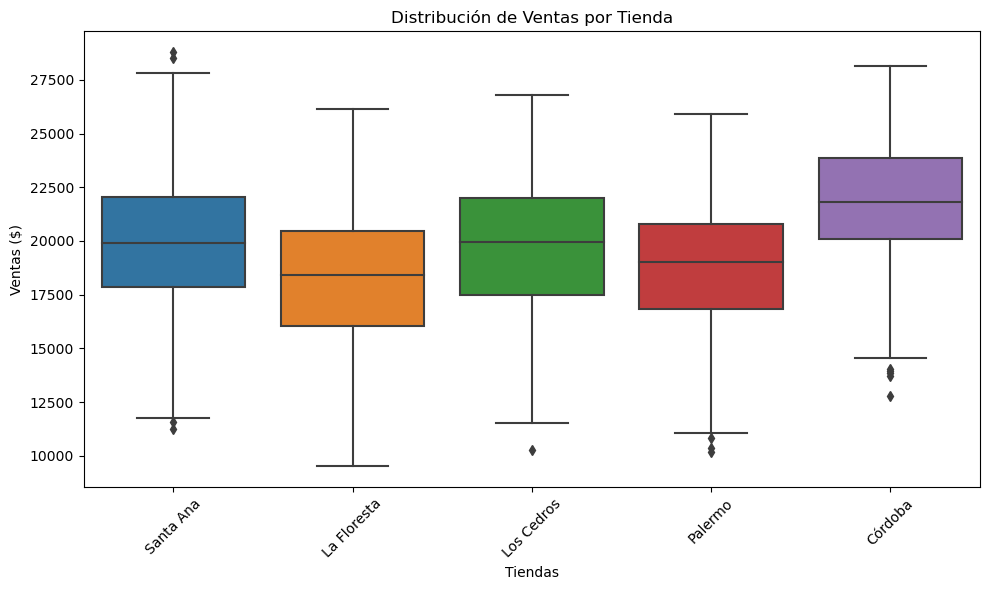
\includegraphics[width=0.7\textwidth]{distribucion_ventas_por_tiendas.png}
    \caption{Diagrama de caja de las ventas de cada tienda}
    \label{fig:ejemplo}
\end{figure}



\subsection{problema 3. Resultados del Análisis Estadístico}

\subsection*{Tiendas Destacadas}
\begin{tabular}{@{}ll@{}}
\toprule
\textbf{La tienda con mayor promedio de ventas es} & C\'ordoba (\$21,784.30) \\
\textbf{La tienda con menor promedio de ventas es} & La Floresta (\$18,049.11) \\
\bottomrule
\end{tabular}


\subsection*{Prueba de Hip\'otesis}

Se plantea la siguiente prueba de hip\'otesis:

\begin{align*}
H_0 &: \text{No hay diferencia significativa entre medias } (\mu_C - \mu_F = 0). \\
H_1 &: \text{Hay diferencia significativa entre medias } (\mu_C - \mu_F \neq 0).
\end{align*}

\subsubsection*{Resultados de la Prueba ANOVA}
La prueba se realiz\'o empleando la funci\'on \texttt{ttest\_ind} de la librer\'ia \texttt{scipy}.

\begin{itemize}
    \item Estad\'istico $t$: 16.2497
    \item Valor $p$: $8.6900 \times 10^{-51}$
\end{itemize}

